\subsection{Francesco Buda} \label{sec:implementation-buda}
Durante lo sviluppo di questo progetto ho lavorato ai seguenti aspetti implementativi del sistema:
\begin{itemize}
    \item Modellazione del tabellone di gioco
    \item Gestione delle mosse dei giocatori tramite PlayingAgent e Controller
    \item Implementazione dei componenti principali dell'interfaccia grafica
    \item Implementazione pagina iniziale dell'applicazione
    \item Implementazione pagina di gioco principale
    \item Minigioco Puzzle per intero
\end{itemize}
di seguito si discutono i dettagli implementativi più rilevanti.

\subsubsection{Modellazione del tabellone di gioco}
Il tabellone di gioco è stato implementato come una case class che contiene due mappe, 
la prima contiene le celle del tabellone indicizzate dalla loro posizione, mentre la seconda contiene
le pedine dei giocatori indicizzate dal loro ID. Di seguito elenco gli aspetti più rilevanti nell'implementazione:
\begin{itemize}
    \item \textbf{BoardBox come algebric data type}\par
    Le celle del gioco possono essere vuote o possono contenere un item al loro interno, per questo sono
    state rappresentate come un algebric data type che somma le due possibilità: emptyBox o FullBox(item).
    \item \textbf{Costruzione del tabellone tramite DSL}\par
    per la costruzione del tabellone di gioco nell'applicazione e nei test si è pensato di implementare un DSL
    sfruttando le funzionalità di Scala, in particolare la possibilità di scrivere metodi in notazione postfissa.
    Questo ha permesso di scrivere il codice in modo molto simile alla rappresentazione grafica del tabellone:
    \begin{lstlisting}[language=Scala]
    \| | O | O | O | O | O | O | 5 | O |
    -> | O | * | * | * | O | * | * | M |
    -> | O | * | * | * | M | * | * | O |
    -> | O | M | O | O | O | O | M | O | O | O |
    -> | O | * | * | * | O | * | * | O | * | O |
    -> | O | * | * | * | O | * | * | O | * | O |
    -> | O | * | * | * | O | * | * | O | * | O |
    -> | O | M | O | O | O | O | M | O | O | O |
    -> | * | * | * | O | * | * | * | * | * | O |
    -> | * | * | * | O | O | M | O | O | O | O |+
      (0, BoardPosition(9, 9)) |+
      (1, BoardPosition(9, 9)) |/
    \end{lstlisting}
    In modo quindi abbastanza intuitivo si può costruire un tabellone nel quale:
    \begin{itemize}
        \item il simbolo \texttt{\textbackslash|} rappresenta l'inizio di un tabellone
        \item il simbolo \texttt{->} rappresenta l'inizio di una nuova riga
        \item il simbolo \texttt{|} rappresenta la separazione tra le celle
        \item il simbolo \texttt{O} rappresenta una cella vuota
        \item il simbolo \texttt{*} rappresenta uno spazio vuoto
        \item il simbolo \texttt{M} rappresenta una cella contenente una monade
        \item un intero rappresenta una cella contenente un piolo il cui prezzo è l'equivalente in numero di monadi dell'intero stesso
        \item il simbolo \texttt{|+} può essere usato per aggiungere pedine in posizioni arbitrarie
        \item il simbolo \texttt{|/} rappresenta la fine del tabellone
    \end{itemize}
\end{itemize}

\subsubsection{Gestione delle mosse dei giocatori tramite PlayingAgent e Controller}
Il componente del controller funge da punto di snodo tra gli agenti dei giocatori (sia che essi siano umani, quindi comandati tramite interfaccia grafica
sia che siano automatizzati) e il resto del sistema. Un aspetto importante da notare è che il controller è l'unico componente dell'architettura principale
a fare uso di mutabilità, tutti gli altri componenti infatti sono oggetti immutabili che vengono aggiornati tramite la creazione di nuove istanze. Ciascuna
tipologia di mossa che sia essa una mossa di ScalaParty o una mossa di un minigioco, è stata modellata come ADT in cui ciascun sottotipo rappresentate
una mossa e contiene i dati necessari per eseguire la mossa stessa.
    \begin{lstlisting}[language=Scala]
    enum PartyMove extends Move:
        case DiceRoll(playerId: Int)
        case Movement(playerId: Int, direction: Direction)
        case StartMinigame
        case Resume
    \end{lstlisting}

\subsubsection{Minigioco Puzzle}
Gli aspetti imlementativi più importanti per quanto riguarda il minigioco Puzzle che ho realizzato sono i seguenti:
\begin{itemize}
    \item \textbf{Creazione ricorsiva di una soluzione valida}\par
    Il fulcro per quanto riguarda la generazione di un insieme di pezzi validi per il minigioco è la funzione \texttt{generateRandomSolution}
    essa prende in ingresso la larghezza, l'altezza del puzzle e la grandezza massima dei pezzi, e genera ricorsivamente un puzzle valido. 
    Si può notare l'utilizzo di un \texttt{for-yeld} per la genrazione di tutte le posizioni iniziali. 
    \begin{lstlisting}[language=Scala]
    (
    for x <- 0 until width
        y <- 0 until height
    yield PuzzlePosition(x, y)
    ).toSet
    \end{lstlisting}
    \item \textbf{Validazione delle soluzioni tramite Prolog}\par
    Per la validazione delle soluzioni dell'utente è stato sfruttato il linguaggio Prolog,
    in particolare è stato implementato un predicato che verifica se una soluzione è valida o meno.
    Il predicato prende in ingresso, l'altezza, la larghezza del puzzle e una soluzione che è stata
    precedentemente mappata in una partizione di un insieme di interi secondo la regola mostrata nella figura \ref{fig:puzzle-prolog-mapping}.
    \begin{figure}[ht!]
        \centering
        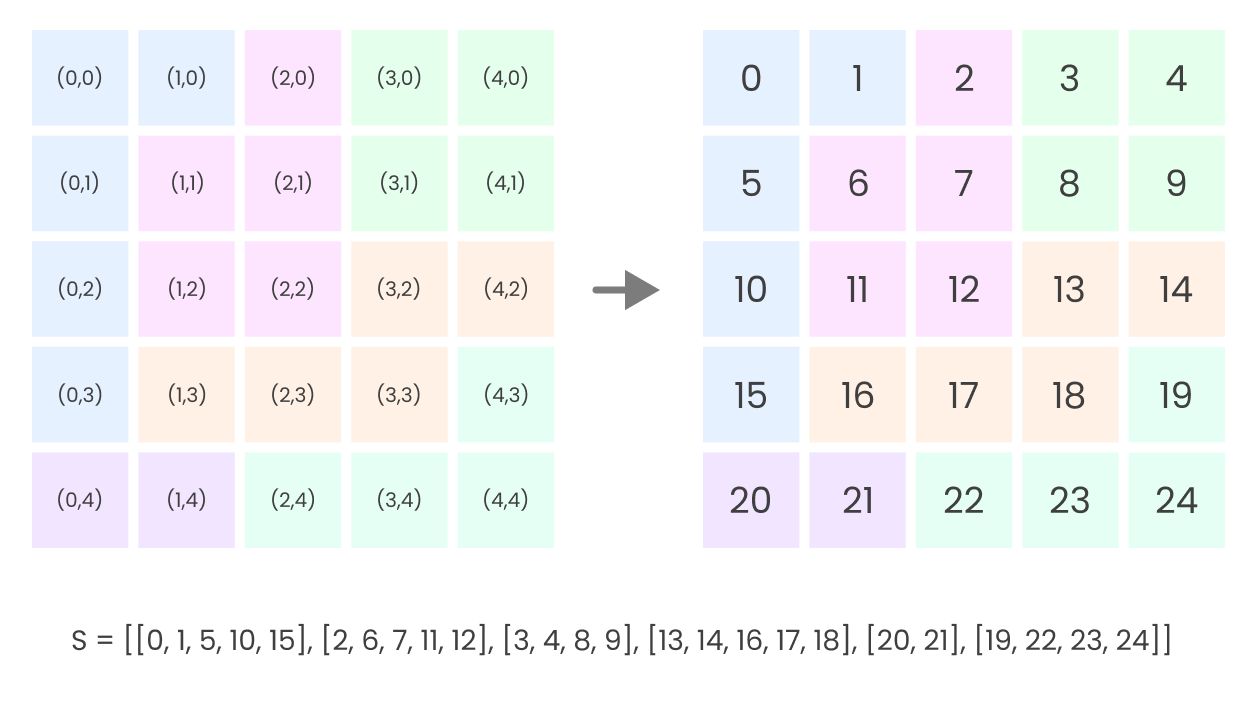
\includegraphics[width=1\textwidth]{figures/puzzlePrologMapping.png}
        \caption{Mapping della soluzione del puzzle in Prolog}
        \label{fig:puzzle-prolog-mapping}
    \end{figure}
    L'algoritmo utilizza la teoria dinamica in Prolog per definire tramite assert le regole di adiacenza tra i numeri,
    successivamente verifica le seguenti tre proprietà che la partizione deve avere:
    \begin{enumerate}
        \item \textbf{Ciascun insieme della partizione rappresenta un pezzo valido}\par
        ovvero ciascun elemento deve essere adiacente ad almeno un altro elemento dell'insieme
        \begin{lstlisting}
    contains_valid_pieces([]).
    contains_valid_pieces([H|T]) :-
	    piece_is_valid(H),
	    contains_valid_pieces(T).

    piece_is_valid(P) :- length(P, 1), !.
    piece_is_valid(P) :-
	    findall(X, (member(X, P), is_adiacent(X, P)), L),
	    length(L, LEN),
	    length(P, N),
	    LEN =:= N.

    is_adiacent(X, P) :-
	    member(Y, P),
	    are_adiacent(X, Y), !.
        \end{lstlisting}
        \item \textbf{Gli insiemi della partizione sono disgiunti}
        \item \textbf{La partizione è completa}\par
        ovvero l'unione degli insiemi che la compongono contiene tutti gli elementi da zero incluso a width*height escluso
    \end{enumerate}
\end{itemize}

